% fig01_f3_spine.tex — the F3 "structure beyond density" spine, all 3 substrates.
% Standalone; compiled by `make figures` (pdflatex). main.tex includes the PDF.
% Data = exact-enumeration verdicts (anima:.verdicts/{906,907,908}/run.txt):
%   A spin-glass : low-f Rbar=31.8, high-f Rbar=50.9  (rescaled R/64 to share [0,1] axis)
%   B category   : low-D Phi=0.775, high-D Phi=0.958  (p=0.4 fixed)
%   C topology   : low-b1 Phi=0.617, high-b1 Phi=0.867 (p=0.4 fixed)
\documentclass[tikz,border=4pt]{standalone}
\usepackage{pgfplots}
\pgfplotsset{compat=1.18}
\begin{document}
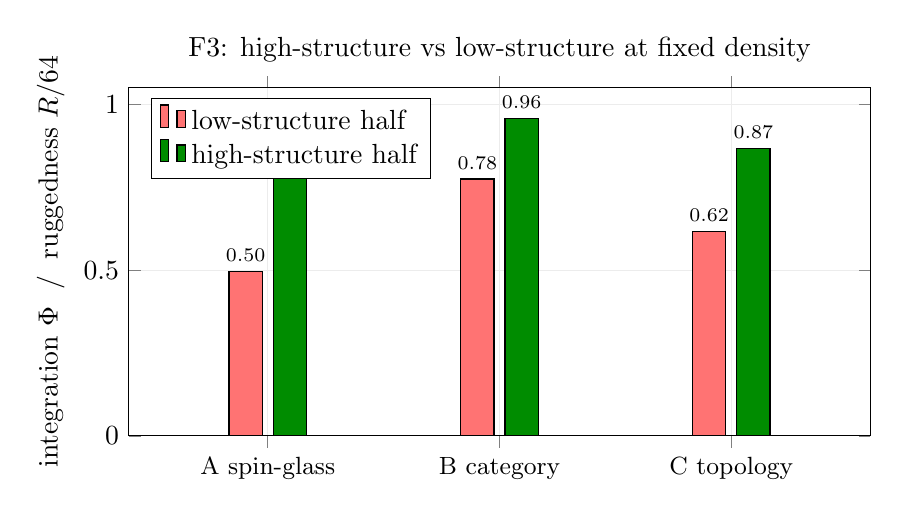
\begin{tikzpicture}
  \begin{axis}[
    width=11cm, height=6cm,
    ybar=4pt, bar width=12pt,
    ymin=0, ymax=1.05,
    ylabel={integration $\Phi$ \;/\; ruggedness $R/64$},
    symbolic x coords={A spin-glass, B category, C topology},
    xtick=data,
    xticklabel style={font=\small},
    nodes near coords, nodes near coords style={font=\scriptsize,
      /pgf/number format/.cd, fixed, fixed zerofill, precision=2},
    enlarge x limits=0.3,
    legend pos=north west, legend cell align=left,
    grid=both, grid style={gray!15},
    title={F3: high-structure vs low-structure at fixed density},
  ]
    % low-structure half
    \addplot[draw=black, fill=red!55] coordinates {
      (A spin-glass, 0.497) (B category, 0.775) (C topology, 0.617)
    };
    \addlegendentry{low-structure half}
    % high-structure half
    \addplot[draw=black, fill=green!55!black] coordinates {
      (A spin-glass, 0.795) (B category, 0.958) (C topology, 0.867)
    };
    \addlegendentry{high-structure half}
  \end{axis}
\end{tikzpicture}
\end{document}
